\documentclass[twoside]{book}

% Packages required by doxygen
\usepackage{fixltx2e}
\usepackage{calc}
\usepackage{doxygen}
\usepackage[export]{adjustbox} % also loads graphicx
\usepackage{graphicx}
\usepackage[utf8]{inputenc}
\usepackage{makeidx}
\usepackage{multicol}
\usepackage{multirow}
\PassOptionsToPackage{warn}{textcomp}
\usepackage{textcomp}
\usepackage[nointegrals]{wasysym}
\usepackage[table]{xcolor}

% Font selection
\usepackage[T1]{fontenc}
\usepackage[scaled=.90]{helvet}
\usepackage{courier}
\usepackage{amssymb}
\usepackage{sectsty}
\renewcommand{\familydefault}{\sfdefault}
\allsectionsfont{%
  \fontseries{bc}\selectfont%
  \color{darkgray}%
}
\renewcommand{\DoxyLabelFont}{%
  \fontseries{bc}\selectfont%
  \color{darkgray}%
}
\newcommand{\+}{\discretionary{\mbox{\scriptsize$\hookleftarrow$}}{}{}}

% Page & text layout
\usepackage{geometry}
\geometry{%
  a4paper,%
  top=2.5cm,%
  bottom=2.5cm,%
  left=2.5cm,%
  right=2.5cm%
}
\tolerance=750
\hfuzz=15pt
\hbadness=750
\setlength{\emergencystretch}{15pt}
\setlength{\parindent}{0cm}
\setlength{\parskip}{3ex plus 2ex minus 2ex}
\makeatletter
\renewcommand{\paragraph}{%
  \@startsection{paragraph}{4}{0ex}{-1.0ex}{1.0ex}{%
    \normalfont\normalsize\bfseries\SS@parafont%
  }%
}
\renewcommand{\subparagraph}{%
  \@startsection{subparagraph}{5}{0ex}{-1.0ex}{1.0ex}{%
    \normalfont\normalsize\bfseries\SS@subparafont%
  }%
}
\makeatother

% Headers & footers
\usepackage{fancyhdr}
\pagestyle{fancyplain}
\fancyhead[LE]{\fancyplain{}{\bfseries\thepage}}
\fancyhead[CE]{\fancyplain{}{}}
\fancyhead[RE]{\fancyplain{}{\bfseries\leftmark}}
\fancyhead[LO]{\fancyplain{}{\bfseries\rightmark}}
\fancyhead[CO]{\fancyplain{}{}}
\fancyhead[RO]{\fancyplain{}{\bfseries\thepage}}
\fancyfoot[LE]{\fancyplain{}{}}
\fancyfoot[CE]{\fancyplain{}{}}
\fancyfoot[RE]{\fancyplain{}{\bfseries\scriptsize Generated by Doxygen }}
\fancyfoot[LO]{\fancyplain{}{\bfseries\scriptsize Generated by Doxygen }}
\fancyfoot[CO]{\fancyplain{}{}}
\fancyfoot[RO]{\fancyplain{}{}}
\renewcommand{\footrulewidth}{0.4pt}
\renewcommand{\chaptermark}[1]{%
  \markboth{#1}{}%
}
\renewcommand{\sectionmark}[1]{%
  \markright{\thesection\ #1}%
}

% Indices & bibliography
\usepackage{natbib}
\usepackage[titles]{tocloft}
\setcounter{tocdepth}{3}
\setcounter{secnumdepth}{5}
\makeindex

% Hyperlinks (required, but should be loaded last)
\usepackage{ifpdf}
\ifpdf
  \usepackage[pdftex,pagebackref=true]{hyperref}
\else
  \usepackage[ps2pdf,pagebackref=true]{hyperref}
\fi
\hypersetup{%
  colorlinks=true,%
  linkcolor=blue,%
  citecolor=blue,%
  unicode%
}

% Custom commands
\newcommand{\clearemptydoublepage}{%
  \newpage{\pagestyle{empty}\cleardoublepage}%
}

\usepackage{caption}
\captionsetup{labelsep=space,justification=centering,font={bf},singlelinecheck=off,skip=4pt,position=top}

%===== C O N T E N T S =====

\begin{document}

% Titlepage & ToC
\hypersetup{pageanchor=false,
             bookmarksnumbered=true,
             pdfencoding=unicode
            }
\pagenumbering{alph}
\begin{titlepage}
\vspace*{7cm}
\begin{center}%
{\Large My Project }\\
\vspace*{1cm}
{\large Generated by Doxygen 1.8.13}\\
\end{center}
\end{titlepage}
\clearemptydoublepage
\pagenumbering{roman}
\tableofcontents
\clearemptydoublepage
\pagenumbering{arabic}
\hypersetup{pageanchor=true}

%--- Begin generated contents ---
\chapter{L\+I2-\/\+P\+L8-\/\+Grp12}
\label{md_README}
\Hypertarget{md_README}
Projeto no âmbito da disciplina de Laboratórios de Informática 2. O objetivo é desenvolver o jogo \char`\"{}\+Rastros\char`\"{} na linguagem C. Projeto realizado por\+: Laura Nunes Rodrigues a93169; Luís Miguel Teixeira Fernandes a88539; Mariana Filipa da Silva Rodrigues a93306. Alunos do P\+L8, grupo 12. 
\chapter{Class Index}
\section{Class List}
Here are the classes, structs, unions and interfaces with brief descriptions\+:\begin{DoxyCompactList}
\item\contentsline{section}{\hyperlink{structCOORDENADA}{C\+O\+O\+R\+D\+E\+N\+A\+DA} \\*Tipo de dados para as coordenadas }{\pageref{structCOORDENADA}}{}
\item\contentsline{section}{\hyperlink{structESTADO}{E\+S\+T\+A\+DO} \\*Tipo de dados para o estado }{\pageref{structESTADO}}{}
\item\contentsline{section}{\hyperlink{structJOGADA}{J\+O\+G\+A\+DA} \\*Tipo de dados para a jogada }{\pageref{structJOGADA}}{}
\end{DoxyCompactList}

\chapter{File Index}
\section{File List}
Here is a list of all documented files with brief descriptions\+:\begin{DoxyCompactList}
\item\contentsline{section}{\hyperlink{Camada__dados_8h}{Camada\+\_\+dados.\+h} }{\pageref{Camada__dados_8h}}{}
\item\contentsline{section}{\hyperlink{Camada__Interface_8h}{Camada\+\_\+\+Interface.\+h} }{\pageref{Camada__Interface_8h}}{}
\item\contentsline{section}{{\bfseries Funcoes\+\_\+\+Ficheiro.\+h} }{\pageref{Funcoes__Ficheiro_8h}}{}
\item\contentsline{section}{\hyperlink{Logica__Programa_8h}{Logica\+\_\+\+Programa.\+h} }{\pageref{Logica__Programa_8h}}{}
\end{DoxyCompactList}

\chapter{Class Documentation}
\hypertarget{structCOORDENADA}{}\section{C\+O\+O\+R\+D\+E\+N\+A\+DA Struct Reference}
\label{structCOORDENADA}\index{C\+O\+O\+R\+D\+E\+N\+A\+DA@{C\+O\+O\+R\+D\+E\+N\+A\+DA}}
\subsection*{Public Attributes}
\begin{DoxyCompactItemize}
\item 
\mbox{\Hypertarget{structCOORDENADA_adfbc8d4856ce807139fdf62e00aed29a}\label{structCOORDENADA_adfbc8d4856ce807139fdf62e00aed29a}} 
int {\bfseries coluna}
\item 
\mbox{\Hypertarget{structCOORDENADA_aefe14bcc5a066ac3b21500cc3d28c06f}\label{structCOORDENADA_aefe14bcc5a066ac3b21500cc3d28c06f}} 
int {\bfseries linha}
\end{DoxyCompactItemize}


The documentation for this struct was generated from the following file\+:\begin{DoxyCompactItemize}
\item 
Camada\+\_\+dados.\+h\end{DoxyCompactItemize}

\hypertarget{structESTADO}{}\section{E\+S\+T\+A\+DO Struct Reference}
\label{structESTADO}\index{E\+S\+T\+A\+DO@{E\+S\+T\+A\+DO}}


Tipo de dados para o estado.  




{\ttfamily \#include $<$Camada\+\_\+dados.\+h$>$}



Collaboration diagram for E\+S\+T\+A\+DO\+:
\nopagebreak
\begin{figure}[H]
\begin{center}
\leavevmode
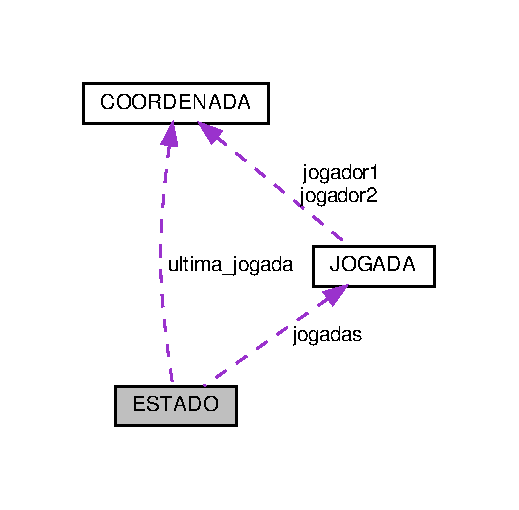
\includegraphics[width=249pt]{structESTADO__coll__graph}
\end{center}
\end{figure}
\subsection*{Public Attributes}
\begin{DoxyCompactItemize}
\item 
\hyperlink{Camada__dados_8h_aba91601f16d4c485b2d9b8c429f27039}{C\+A\+SA} \hyperlink{structESTADO_ab56f0f1be16954d3768b4174d14c087d}{tab} \mbox{[}8\mbox{]}\mbox{[}8\mbox{]}
\item 
\hyperlink{structCOORDENADA}{C\+O\+O\+R\+D\+E\+N\+A\+DA} \hyperlink{structESTADO_a4896a5c5c1f40b43fb795623327e3f47}{ultima\+\_\+jogada}
\item 
\hyperlink{Camada__dados_8h_a94c221d29a1760f008b7834093259b7d}{J\+O\+G\+A\+D\+AS} \hyperlink{structESTADO_afae43b87a488fad0f2b56a18bad31d18}{jogadas}
\item 
int \hyperlink{structESTADO_a261495728744647e618b4e623f5a4b7a}{num\+\_\+jogadas}
\item 
int \hyperlink{structESTADO_a5dd28e2e68b7aef2b6b7ea88e02eff58}{jogador\+\_\+atual}
\item 
int \hyperlink{structESTADO_a8d478f3546194c1666c6e390c8aaf1cb}{num\+\_\+movimentos}
\item 
int \hyperlink{structESTADO_aceee2863ecd183efc410fb079a576cba}{alt\+\_\+pos}
\end{DoxyCompactItemize}


\subsection{Detailed Description}
Tipo de dados para o estado. 

\subsection{Member Data Documentation}
\mbox{\Hypertarget{structESTADO_aceee2863ecd183efc410fb079a576cba}\label{structESTADO_aceee2863ecd183efc410fb079a576cba}} 
\index{E\+S\+T\+A\+DO@{E\+S\+T\+A\+DO}!alt\+\_\+pos@{alt\+\_\+pos}}
\index{alt\+\_\+pos@{alt\+\_\+pos}!E\+S\+T\+A\+DO@{E\+S\+T\+A\+DO}}
\subsubsection{\texorpdfstring{alt\+\_\+pos}{alt\_pos}}
{\footnotesize\ttfamily int E\+S\+T\+A\+D\+O\+::alt\+\_\+pos}

Jogada anterior foi pos \mbox{\Hypertarget{structESTADO_afae43b87a488fad0f2b56a18bad31d18}\label{structESTADO_afae43b87a488fad0f2b56a18bad31d18}} 
\index{E\+S\+T\+A\+DO@{E\+S\+T\+A\+DO}!jogadas@{jogadas}}
\index{jogadas@{jogadas}!E\+S\+T\+A\+DO@{E\+S\+T\+A\+DO}}
\subsubsection{\texorpdfstring{jogadas}{jogadas}}
{\footnotesize\ttfamily \hyperlink{Camada__dados_8h_a94c221d29a1760f008b7834093259b7d}{J\+O\+G\+A\+D\+AS} E\+S\+T\+A\+D\+O\+::jogadas}

As jogadas \mbox{\Hypertarget{structESTADO_a5dd28e2e68b7aef2b6b7ea88e02eff58}\label{structESTADO_a5dd28e2e68b7aef2b6b7ea88e02eff58}} 
\index{E\+S\+T\+A\+DO@{E\+S\+T\+A\+DO}!jogador\+\_\+atual@{jogador\+\_\+atual}}
\index{jogador\+\_\+atual@{jogador\+\_\+atual}!E\+S\+T\+A\+DO@{E\+S\+T\+A\+DO}}
\subsubsection{\texorpdfstring{jogador\+\_\+atual}{jogador\_atual}}
{\footnotesize\ttfamily int E\+S\+T\+A\+D\+O\+::jogador\+\_\+atual}

O jogador atual \mbox{\Hypertarget{structESTADO_a261495728744647e618b4e623f5a4b7a}\label{structESTADO_a261495728744647e618b4e623f5a4b7a}} 
\index{E\+S\+T\+A\+DO@{E\+S\+T\+A\+DO}!num\+\_\+jogadas@{num\+\_\+jogadas}}
\index{num\+\_\+jogadas@{num\+\_\+jogadas}!E\+S\+T\+A\+DO@{E\+S\+T\+A\+DO}}
\subsubsection{\texorpdfstring{num\+\_\+jogadas}{num\_jogadas}}
{\footnotesize\ttfamily int E\+S\+T\+A\+D\+O\+::num\+\_\+jogadas}

O número das jogadas, usado no prompt \mbox{\Hypertarget{structESTADO_a8d478f3546194c1666c6e390c8aaf1cb}\label{structESTADO_a8d478f3546194c1666c6e390c8aaf1cb}} 
\index{E\+S\+T\+A\+DO@{E\+S\+T\+A\+DO}!num\+\_\+movimentos@{num\+\_\+movimentos}}
\index{num\+\_\+movimentos@{num\+\_\+movimentos}!E\+S\+T\+A\+DO@{E\+S\+T\+A\+DO}}
\subsubsection{\texorpdfstring{num\+\_\+movimentos}{num\_movimentos}}
{\footnotesize\ttfamily int E\+S\+T\+A\+D\+O\+::num\+\_\+movimentos}

Número de movimentos \mbox{\Hypertarget{structESTADO_ab56f0f1be16954d3768b4174d14c087d}\label{structESTADO_ab56f0f1be16954d3768b4174d14c087d}} 
\index{E\+S\+T\+A\+DO@{E\+S\+T\+A\+DO}!tab@{tab}}
\index{tab@{tab}!E\+S\+T\+A\+DO@{E\+S\+T\+A\+DO}}
\subsubsection{\texorpdfstring{tab}{tab}}
{\footnotesize\ttfamily \hyperlink{Camada__dados_8h_aba91601f16d4c485b2d9b8c429f27039}{C\+A\+SA} E\+S\+T\+A\+D\+O\+::tab\mbox{[}8\mbox{]}\mbox{[}8\mbox{]}}

O tabuleiro \mbox{\Hypertarget{structESTADO_a4896a5c5c1f40b43fb795623327e3f47}\label{structESTADO_a4896a5c5c1f40b43fb795623327e3f47}} 
\index{E\+S\+T\+A\+DO@{E\+S\+T\+A\+DO}!ultima\+\_\+jogada@{ultima\+\_\+jogada}}
\index{ultima\+\_\+jogada@{ultima\+\_\+jogada}!E\+S\+T\+A\+DO@{E\+S\+T\+A\+DO}}
\subsubsection{\texorpdfstring{ultima\+\_\+jogada}{ultima\_jogada}}
{\footnotesize\ttfamily \hyperlink{structCOORDENADA}{C\+O\+O\+R\+D\+E\+N\+A\+DA} E\+S\+T\+A\+D\+O\+::ultima\+\_\+jogada}

A coordenada da última jogada 

The documentation for this struct was generated from the following file\+:\begin{DoxyCompactItemize}
\item 
\hyperlink{Camada__dados_8h}{Camada\+\_\+dados.\+h}\end{DoxyCompactItemize}

\hypertarget{structJOGADA}{}\section{J\+O\+G\+A\+DA Struct Reference}
\label{structJOGADA}\index{J\+O\+G\+A\+DA@{J\+O\+G\+A\+DA}}


Tipo de dados para a jogada.  




{\ttfamily \#include $<$Camada\+\_\+dados.\+h$>$}



Collaboration diagram for J\+O\+G\+A\+DA\+:
\nopagebreak
\begin{figure}[H]
\begin{center}
\leavevmode
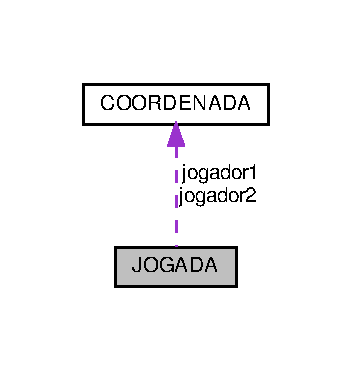
\includegraphics[width=169pt]{structJOGADA__coll__graph}
\end{center}
\end{figure}
\subsection*{Public Attributes}
\begin{DoxyCompactItemize}
\item 
\mbox{\Hypertarget{structJOGADA_a93d9306cb0c49b66b7d9a615bffe0149}\label{structJOGADA_a93d9306cb0c49b66b7d9a615bffe0149}} 
\hyperlink{structCOORDENADA}{C\+O\+O\+R\+D\+E\+N\+A\+DA} {\bfseries jogador1}
\item 
\mbox{\Hypertarget{structJOGADA_ab46b16dfbdc7f2af9430c8dcdac0914b}\label{structJOGADA_ab46b16dfbdc7f2af9430c8dcdac0914b}} 
\hyperlink{structCOORDENADA}{C\+O\+O\+R\+D\+E\+N\+A\+DA} {\bfseries jogador2}
\end{DoxyCompactItemize}


\subsection{Detailed Description}
Tipo de dados para a jogada. 

The documentation for this struct was generated from the following file\+:\begin{DoxyCompactItemize}
\item 
\hyperlink{Camada__dados_8h}{Camada\+\_\+dados.\+h}\end{DoxyCompactItemize}

\chapter{File Documentation}
\hypertarget{Camada__dados_8h}{}\section{Camada\+\_\+dados.\+h File Reference}
\label{Camada__dados_8h}\index{Camada\+\_\+dados.\+h@{Camada\+\_\+dados.\+h}}
This graph shows which files directly or indirectly include this file\+:
\nopagebreak
\begin{figure}[H]
\begin{center}
\leavevmode
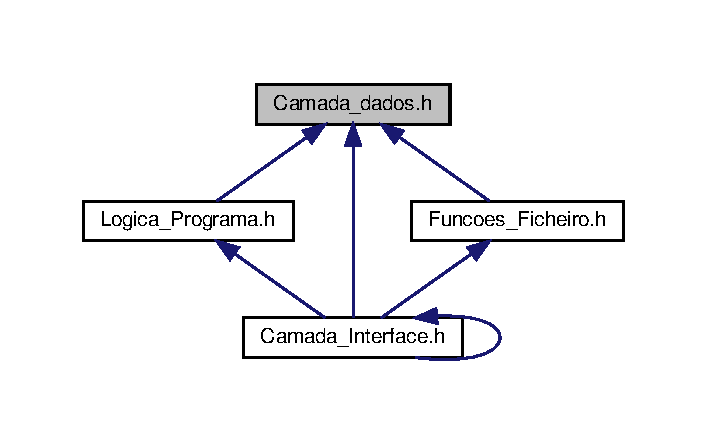
\includegraphics[width=340pt]{Camada__dados_8h__dep__incl}
\end{center}
\end{figure}
\subsection*{Classes}
\begin{DoxyCompactItemize}
\item 
struct \hyperlink{structCOORDENADA}{C\+O\+O\+R\+D\+E\+N\+A\+DA}
\begin{DoxyCompactList}\small\item\em Tipo de dados para as coordenadas. \end{DoxyCompactList}\item 
struct \hyperlink{structJOGADA}{J\+O\+G\+A\+DA}
\begin{DoxyCompactList}\small\item\em Tipo de dados para a jogada. \end{DoxyCompactList}\item 
struct \hyperlink{structESTADO}{E\+S\+T\+A\+DO}
\begin{DoxyCompactList}\small\item\em Tipo de dados para o estado. \end{DoxyCompactList}\end{DoxyCompactItemize}
\subsection*{Typedefs}
\begin{DoxyCompactItemize}
\item 
\mbox{\Hypertarget{Camada__dados_8h_a94c221d29a1760f008b7834093259b7d}\label{Camada__dados_8h_a94c221d29a1760f008b7834093259b7d}} 
typedef \hyperlink{structJOGADA}{J\+O\+G\+A\+DA} \hyperlink{Camada__dados_8h_a94c221d29a1760f008b7834093259b7d}{J\+O\+G\+A\+D\+AS}\mbox{[}32\mbox{]}
\begin{DoxyCompactList}\small\item\em Tipo de dados para as jogadas. \end{DoxyCompactList}\end{DoxyCompactItemize}
\subsection*{Enumerations}
\begin{DoxyCompactItemize}
\item 
\mbox{\Hypertarget{Camada__dados_8h_aba91601f16d4c485b2d9b8c429f27039}\label{Camada__dados_8h_aba91601f16d4c485b2d9b8c429f27039}} 
enum \hyperlink{Camada__dados_8h_aba91601f16d4c485b2d9b8c429f27039}{C\+A\+SA} \{ \newline
{\bfseries V\+A\+Z\+IO}, 
{\bfseries B\+R\+A\+N\+CA}, 
{\bfseries P\+R\+E\+TA}, 
{\bfseries UM}, 
\newline
{\bfseries D\+O\+IS}
 \}\begin{DoxyCompactList}\small\item\em Tipo de dados para a casa. \end{DoxyCompactList}
\end{DoxyCompactItemize}
\subsection*{Functions}
\begin{DoxyCompactItemize}
\item 
\hyperlink{structESTADO}{E\+S\+T\+A\+DO} $\ast$ \hyperlink{Camada__dados_8h_a7e0c7e26fb685d9ab501e19b05e6954f}{inicializar\+\_\+estado} ()
\begin{DoxyCompactList}\small\item\em Inicializa o valor do estado Esta função inicializa o valor do estado. Isso implica o tabuleiro ser colocado na posição inicial e todos os campos do estado estarem com o valor por omissão. \end{DoxyCompactList}\item 
int \hyperlink{Camada__dados_8h_ad6e326e4ffa57ca1ae0c75377ecefc8c}{obter\+\_\+jogador\+\_\+atual} (\hyperlink{structESTADO}{E\+S\+T\+A\+DO} $\ast$estado)
\begin{DoxyCompactList}\small\item\em Permite obter o número do jogador atual. \end{DoxyCompactList}\item 
int \hyperlink{Camada__dados_8h_a6cd0b387bdee9e18003c78852394aa63}{obter\+\_\+numero\+\_\+de\+\_\+jogadas} (\hyperlink{structESTADO}{E\+S\+T\+A\+DO} $\ast$estado)
\begin{DoxyCompactList}\small\item\em Permite obter quantas jogadas foram efetuadas. \end{DoxyCompactList}\item 
\hyperlink{structCOORDENADA}{C\+O\+O\+R\+D\+E\+N\+A\+DA} \hyperlink{Camada__dados_8h_ace0c68928df252cb64d870aac975d0ac}{troca\+\_\+ordem} (\hyperlink{structCOORDENADA}{C\+O\+O\+R\+D\+E\+N\+A\+DA} c)
\begin{DoxyCompactList}\small\item\em Função que troca a coluna pela linha e vice-\/versa. \end{DoxyCompactList}\item 
\hyperlink{Camada__dados_8h_aba91601f16d4c485b2d9b8c429f27039}{C\+A\+SA} \hyperlink{Camada__dados_8h_a6faa68373203923729ed38657aa0f768}{obter\+\_\+estado\+\_\+casa} (\hyperlink{structESTADO}{E\+S\+T\+A\+DO} $\ast$e, \hyperlink{structCOORDENADA}{C\+O\+O\+R\+D\+E\+N\+A\+DA} c)
\begin{DoxyCompactList}\small\item\em Devolve o estado de uma casa. \end{DoxyCompactList}\item 
\hyperlink{structCOORDENADA}{C\+O\+O\+R\+D\+E\+N\+A\+DA} \hyperlink{Camada__dados_8h_a002d7b97f6e1f8bfa2b50efbe03d62bf}{obter\+\_\+ultima\+\_\+jogada} (\hyperlink{structESTADO}{E\+S\+T\+A\+DO} $\ast$estado)
\begin{DoxyCompactList}\small\item\em Devolve a coordenada da última jogada. \end{DoxyCompactList}\item 
int \hyperlink{Camada__dados_8h_a850a8b148b1e314ad75d824163121682}{obter\+\_\+num\+\_\+mov} (\hyperlink{structESTADO}{E\+S\+T\+A\+DO} $\ast$e)
\begin{DoxyCompactList}\small\item\em Devolve o número de movimentos feitos. \end{DoxyCompactList}\item 
\hyperlink{structCOORDENADA}{C\+O\+O\+R\+D\+E\+N\+A\+DA} \hyperlink{Camada__dados_8h_af1d86e313217ba928c29f99996731a27}{obter\+\_\+jogada} (\hyperlink{structESTADO}{E\+S\+T\+A\+DO} $\ast$e, int njogada, int jogador)
\begin{DoxyCompactList}\small\item\em Permite obter a jogada. \end{DoxyCompactList}\item 
int \hyperlink{Camada__dados_8h_a36fa4b2606965343116e3a271246be29}{obter\+\_\+pos} (\hyperlink{structESTADO}{E\+S\+T\+A\+DO} $\ast$e)
\begin{DoxyCompactList}\small\item\em Permite obter o valor da variavel alt\+\_\+pos. \end{DoxyCompactList}\item 
void \hyperlink{Camada__dados_8h_ae6cf63201c192db12d418b36a4843af4}{aumenta\+\_\+pos} (\hyperlink{structESTADO}{E\+S\+T\+A\+DO} $\ast$e, int i)
\begin{DoxyCompactList}\small\item\em Altera a variavel da alt\+\_\+pos e incrementa um. \end{DoxyCompactList}\item 
void \hyperlink{Camada__dados_8h_afdd0e77e8a9642285de9f2ec590283f1}{altera\+\_\+pos} (\hyperlink{structESTADO}{E\+S\+T\+A\+DO} $\ast$e)
\begin{DoxyCompactList}\small\item\em Permite alterar o valor da variavel alt\+\_\+pos. \end{DoxyCompactList}\item 
void \hyperlink{Camada__dados_8h_a7bae87bdf01aa122773a33c56f08dea8}{altera\+\_\+tabuleiro} (\hyperlink{structESTADO}{E\+S\+T\+A\+DO} $\ast$estado, \hyperlink{structCOORDENADA}{C\+O\+O\+R\+D\+E\+N\+A\+DA} c)
\begin{DoxyCompactList}\small\item\em Altera o tabuleiro. \end{DoxyCompactList}\item 
void \hyperlink{Camada__dados_8h_a8828526e2c272cd90636cc20be682929}{altera\+\_\+ultimajogada} (\hyperlink{structESTADO}{E\+S\+T\+A\+DO} $\ast$e, \hyperlink{structCOORDENADA}{C\+O\+O\+R\+D\+E\+N\+A\+DA} c)
\begin{DoxyCompactList}\small\item\em Altera a última jogada, para a coordenada dada. \end{DoxyCompactList}\item 
void \hyperlink{Camada__dados_8h_accd4328aa4c98be72e5e4749d27993e1}{altera\+\_\+jogadas} (\hyperlink{structESTADO}{E\+S\+T\+A\+DO} $\ast$e, \hyperlink{structCOORDENADA}{C\+O\+O\+R\+D\+E\+N\+A\+DA} c)
\begin{DoxyCompactList}\small\item\em Altera as jogadas. \end{DoxyCompactList}\item 
void \hyperlink{Camada__dados_8h_a7bec07cb8d6a3dbe395f8fa529eba0db}{altera\+\_\+jogadoratual} (\hyperlink{structESTADO}{E\+S\+T\+A\+DO} $\ast$e)
\begin{DoxyCompactList}\small\item\em Altera o jogador atual. \end{DoxyCompactList}\item 
void \hyperlink{Camada__dados_8h_ac316f3f24c4b7f50736121bd47a68e70}{altera\+\_\+num\+\_\+mov} (\hyperlink{structESTADO}{E\+S\+T\+A\+DO} $\ast$e, int n\+\_\+mov)
\begin{DoxyCompactList}\small\item\em Aumenta o numero de movimentos. \end{DoxyCompactList}\item 
void \hyperlink{Camada__dados_8h_a6cad793a2982ab22e2099003b569d6b2}{altera\+\_\+numjogadas} (\hyperlink{structESTADO}{E\+S\+T\+A\+DO} $\ast$e)
\begin{DoxyCompactList}\small\item\em Aumenta o numero de jogadas. \end{DoxyCompactList}\item 
void \hyperlink{Camada__dados_8h_a7a5f5de11e3d418ba36aebde7057a403}{faz\+\_\+primeira\+\_\+jogada} (\hyperlink{structESTADO}{E\+S\+T\+A\+DO} $\ast$e)
\begin{DoxyCompactList}\small\item\em Altera detalhes do estado inicial. \end{DoxyCompactList}\item 
void \hyperlink{Camada__dados_8h_a7e0b4894c0754174beaeec212f7a7819}{altera\+\_\+estado} (\hyperlink{structESTADO}{E\+S\+T\+A\+DO} $\ast$e, \hyperlink{structCOORDENADA}{C\+O\+O\+R\+D\+E\+N\+A\+DA} c)
\begin{DoxyCompactList}\small\item\em Altera o estado. \end{DoxyCompactList}\end{DoxyCompactItemize}


\subsection{Detailed Description}
Definição do estado e das funções que o manipulam 

\subsection{Function Documentation}
\mbox{\Hypertarget{Camada__dados_8h_a7e0b4894c0754174beaeec212f7a7819}\label{Camada__dados_8h_a7e0b4894c0754174beaeec212f7a7819}} 
\index{Camada\+\_\+dados.\+h@{Camada\+\_\+dados.\+h}!altera\+\_\+estado@{altera\+\_\+estado}}
\index{altera\+\_\+estado@{altera\+\_\+estado}!Camada\+\_\+dados.\+h@{Camada\+\_\+dados.\+h}}
\subsubsection{\texorpdfstring{altera\+\_\+estado()}{altera\_estado()}}
{\footnotesize\ttfamily void altera\+\_\+estado (\begin{DoxyParamCaption}\item[{\hyperlink{structESTADO}{E\+S\+T\+A\+DO} $\ast$}]{e,  }\item[{\hyperlink{structCOORDENADA}{C\+O\+O\+R\+D\+E\+N\+A\+DA}}]{c }\end{DoxyParamCaption})}



Altera o estado. 


\begin{DoxyParams}{Parameters}
{\em e} & Apontador para o estado \\
\hline
{\em c} & A coordenada \\
\hline
\end{DoxyParams}
\mbox{\Hypertarget{Camada__dados_8h_accd4328aa4c98be72e5e4749d27993e1}\label{Camada__dados_8h_accd4328aa4c98be72e5e4749d27993e1}} 
\index{Camada\+\_\+dados.\+h@{Camada\+\_\+dados.\+h}!altera\+\_\+jogadas@{altera\+\_\+jogadas}}
\index{altera\+\_\+jogadas@{altera\+\_\+jogadas}!Camada\+\_\+dados.\+h@{Camada\+\_\+dados.\+h}}
\subsubsection{\texorpdfstring{altera\+\_\+jogadas()}{altera\_jogadas()}}
{\footnotesize\ttfamily void altera\+\_\+jogadas (\begin{DoxyParamCaption}\item[{\hyperlink{structESTADO}{E\+S\+T\+A\+DO} $\ast$}]{e,  }\item[{\hyperlink{structCOORDENADA}{C\+O\+O\+R\+D\+E\+N\+A\+DA}}]{c }\end{DoxyParamCaption})}



Altera as jogadas. 


\begin{DoxyParams}{Parameters}
{\em e} & Apontador para o estado \\
\hline
{\em c} & A coordenada \\
\hline
\end{DoxyParams}
\mbox{\Hypertarget{Camada__dados_8h_a7bec07cb8d6a3dbe395f8fa529eba0db}\label{Camada__dados_8h_a7bec07cb8d6a3dbe395f8fa529eba0db}} 
\index{Camada\+\_\+dados.\+h@{Camada\+\_\+dados.\+h}!altera\+\_\+jogadoratual@{altera\+\_\+jogadoratual}}
\index{altera\+\_\+jogadoratual@{altera\+\_\+jogadoratual}!Camada\+\_\+dados.\+h@{Camada\+\_\+dados.\+h}}
\subsubsection{\texorpdfstring{altera\+\_\+jogadoratual()}{altera\_jogadoratual()}}
{\footnotesize\ttfamily void altera\+\_\+jogadoratual (\begin{DoxyParamCaption}\item[{\hyperlink{structESTADO}{E\+S\+T\+A\+DO} $\ast$}]{e }\end{DoxyParamCaption})}



Altera o jogador atual. 


\begin{DoxyParams}{Parameters}
{\em e} & Apontador para o estado \\
\hline
\end{DoxyParams}
\mbox{\Hypertarget{Camada__dados_8h_ac316f3f24c4b7f50736121bd47a68e70}\label{Camada__dados_8h_ac316f3f24c4b7f50736121bd47a68e70}} 
\index{Camada\+\_\+dados.\+h@{Camada\+\_\+dados.\+h}!altera\+\_\+num\+\_\+mov@{altera\+\_\+num\+\_\+mov}}
\index{altera\+\_\+num\+\_\+mov@{altera\+\_\+num\+\_\+mov}!Camada\+\_\+dados.\+h@{Camada\+\_\+dados.\+h}}
\subsubsection{\texorpdfstring{altera\+\_\+num\+\_\+mov()}{altera\_num\_mov()}}
{\footnotesize\ttfamily void altera\+\_\+num\+\_\+mov (\begin{DoxyParamCaption}\item[{\hyperlink{structESTADO}{E\+S\+T\+A\+DO} $\ast$}]{e,  }\item[{int}]{n\+\_\+mov }\end{DoxyParamCaption})}



Aumenta o numero de movimentos. 


\begin{DoxyParams}{Parameters}
{\em e} & Apontador para o estado \\
\hline
{\em n\+\_\+mov} & O inteiro \\
\hline
\end{DoxyParams}
\mbox{\Hypertarget{Camada__dados_8h_a6cad793a2982ab22e2099003b569d6b2}\label{Camada__dados_8h_a6cad793a2982ab22e2099003b569d6b2}} 
\index{Camada\+\_\+dados.\+h@{Camada\+\_\+dados.\+h}!altera\+\_\+numjogadas@{altera\+\_\+numjogadas}}
\index{altera\+\_\+numjogadas@{altera\+\_\+numjogadas}!Camada\+\_\+dados.\+h@{Camada\+\_\+dados.\+h}}
\subsubsection{\texorpdfstring{altera\+\_\+numjogadas()}{altera\_numjogadas()}}
{\footnotesize\ttfamily void altera\+\_\+numjogadas (\begin{DoxyParamCaption}\item[{\hyperlink{structESTADO}{E\+S\+T\+A\+DO} $\ast$}]{e }\end{DoxyParamCaption})}



Aumenta o numero de jogadas. 


\begin{DoxyParams}{Parameters}
{\em e} & Apontador para o estado \\
\hline
\end{DoxyParams}
\mbox{\Hypertarget{Camada__dados_8h_afdd0e77e8a9642285de9f2ec590283f1}\label{Camada__dados_8h_afdd0e77e8a9642285de9f2ec590283f1}} 
\index{Camada\+\_\+dados.\+h@{Camada\+\_\+dados.\+h}!altera\+\_\+pos@{altera\+\_\+pos}}
\index{altera\+\_\+pos@{altera\+\_\+pos}!Camada\+\_\+dados.\+h@{Camada\+\_\+dados.\+h}}
\subsubsection{\texorpdfstring{altera\+\_\+pos()}{altera\_pos()}}
{\footnotesize\ttfamily void altera\+\_\+pos (\begin{DoxyParamCaption}\item[{\hyperlink{structESTADO}{E\+S\+T\+A\+DO} $\ast$}]{e }\end{DoxyParamCaption})}



Permite alterar o valor da variavel alt\+\_\+pos. 


\begin{DoxyParams}{Parameters}
{\em e} & Apontador para o estado \\
\hline
\end{DoxyParams}
\mbox{\Hypertarget{Camada__dados_8h_a7bae87bdf01aa122773a33c56f08dea8}\label{Camada__dados_8h_a7bae87bdf01aa122773a33c56f08dea8}} 
\index{Camada\+\_\+dados.\+h@{Camada\+\_\+dados.\+h}!altera\+\_\+tabuleiro@{altera\+\_\+tabuleiro}}
\index{altera\+\_\+tabuleiro@{altera\+\_\+tabuleiro}!Camada\+\_\+dados.\+h@{Camada\+\_\+dados.\+h}}
\subsubsection{\texorpdfstring{altera\+\_\+tabuleiro()}{altera\_tabuleiro()}}
{\footnotesize\ttfamily void altera\+\_\+tabuleiro (\begin{DoxyParamCaption}\item[{\hyperlink{structESTADO}{E\+S\+T\+A\+DO} $\ast$}]{estado,  }\item[{\hyperlink{structCOORDENADA}{C\+O\+O\+R\+D\+E\+N\+A\+DA}}]{c }\end{DoxyParamCaption})}



Altera o tabuleiro. 


\begin{DoxyParams}{Parameters}
{\em estado} & Apontador para o estado \\
\hline
{\em c} & A coordenada \\
\hline
\end{DoxyParams}
\mbox{\Hypertarget{Camada__dados_8h_a8828526e2c272cd90636cc20be682929}\label{Camada__dados_8h_a8828526e2c272cd90636cc20be682929}} 
\index{Camada\+\_\+dados.\+h@{Camada\+\_\+dados.\+h}!altera\+\_\+ultimajogada@{altera\+\_\+ultimajogada}}
\index{altera\+\_\+ultimajogada@{altera\+\_\+ultimajogada}!Camada\+\_\+dados.\+h@{Camada\+\_\+dados.\+h}}
\subsubsection{\texorpdfstring{altera\+\_\+ultimajogada()}{altera\_ultimajogada()}}
{\footnotesize\ttfamily void altera\+\_\+ultimajogada (\begin{DoxyParamCaption}\item[{\hyperlink{structESTADO}{E\+S\+T\+A\+DO} $\ast$}]{e,  }\item[{\hyperlink{structCOORDENADA}{C\+O\+O\+R\+D\+E\+N\+A\+DA}}]{c }\end{DoxyParamCaption})}



Altera a última jogada, para a coordenada dada. 


\begin{DoxyParams}{Parameters}
{\em e} & Apontador para o estado \\
\hline
{\em c} & A coordenada \\
\hline
\end{DoxyParams}
\mbox{\Hypertarget{Camada__dados_8h_ae6cf63201c192db12d418b36a4843af4}\label{Camada__dados_8h_ae6cf63201c192db12d418b36a4843af4}} 
\index{Camada\+\_\+dados.\+h@{Camada\+\_\+dados.\+h}!aumenta\+\_\+pos@{aumenta\+\_\+pos}}
\index{aumenta\+\_\+pos@{aumenta\+\_\+pos}!Camada\+\_\+dados.\+h@{Camada\+\_\+dados.\+h}}
\subsubsection{\texorpdfstring{aumenta\+\_\+pos()}{aumenta\_pos()}}
{\footnotesize\ttfamily void aumenta\+\_\+pos (\begin{DoxyParamCaption}\item[{\hyperlink{structESTADO}{E\+S\+T\+A\+DO} $\ast$}]{e,  }\item[{int}]{i }\end{DoxyParamCaption})}



Altera a variavel da alt\+\_\+pos e incrementa um. 


\begin{DoxyParams}{Parameters}
{\em e} & Apontador para o estado \\
\hline
{\em i} & Inteiro \\
\hline
\end{DoxyParams}
\mbox{\Hypertarget{Camada__dados_8h_a7a5f5de11e3d418ba36aebde7057a403}\label{Camada__dados_8h_a7a5f5de11e3d418ba36aebde7057a403}} 
\index{Camada\+\_\+dados.\+h@{Camada\+\_\+dados.\+h}!faz\+\_\+primeira\+\_\+jogada@{faz\+\_\+primeira\+\_\+jogada}}
\index{faz\+\_\+primeira\+\_\+jogada@{faz\+\_\+primeira\+\_\+jogada}!Camada\+\_\+dados.\+h@{Camada\+\_\+dados.\+h}}
\subsubsection{\texorpdfstring{faz\+\_\+primeira\+\_\+jogada()}{faz\_primeira\_jogada()}}
{\footnotesize\ttfamily void faz\+\_\+primeira\+\_\+jogada (\begin{DoxyParamCaption}\item[{\hyperlink{structESTADO}{E\+S\+T\+A\+DO} $\ast$}]{e }\end{DoxyParamCaption})}



Altera detalhes do estado inicial. 


\begin{DoxyParams}{Parameters}
{\em estado} & Apontador para o estado \\
\hline
\end{DoxyParams}
\mbox{\Hypertarget{Camada__dados_8h_a7e0c7e26fb685d9ab501e19b05e6954f}\label{Camada__dados_8h_a7e0c7e26fb685d9ab501e19b05e6954f}} 
\index{Camada\+\_\+dados.\+h@{Camada\+\_\+dados.\+h}!inicializar\+\_\+estado@{inicializar\+\_\+estado}}
\index{inicializar\+\_\+estado@{inicializar\+\_\+estado}!Camada\+\_\+dados.\+h@{Camada\+\_\+dados.\+h}}
\subsubsection{\texorpdfstring{inicializar\+\_\+estado()}{inicializar\_estado()}}
{\footnotesize\ttfamily \hyperlink{structESTADO}{E\+S\+T\+A\+DO}$\ast$ inicializar\+\_\+estado (\begin{DoxyParamCaption}{ }\end{DoxyParamCaption})}



Inicializa o valor do estado Esta função inicializa o valor do estado. Isso implica o tabuleiro ser colocado na posição inicial e todos os campos do estado estarem com o valor por omissão. 

\begin{DoxyReturn}{Returns}
O novo estado 
\end{DoxyReturn}
\mbox{\Hypertarget{Camada__dados_8h_a6faa68373203923729ed38657aa0f768}\label{Camada__dados_8h_a6faa68373203923729ed38657aa0f768}} 
\index{Camada\+\_\+dados.\+h@{Camada\+\_\+dados.\+h}!obter\+\_\+estado\+\_\+casa@{obter\+\_\+estado\+\_\+casa}}
\index{obter\+\_\+estado\+\_\+casa@{obter\+\_\+estado\+\_\+casa}!Camada\+\_\+dados.\+h@{Camada\+\_\+dados.\+h}}
\subsubsection{\texorpdfstring{obter\+\_\+estado\+\_\+casa()}{obter\_estado\_casa()}}
{\footnotesize\ttfamily \hyperlink{Camada__dados_8h_aba91601f16d4c485b2d9b8c429f27039}{C\+A\+SA} obter\+\_\+estado\+\_\+casa (\begin{DoxyParamCaption}\item[{\hyperlink{structESTADO}{E\+S\+T\+A\+DO} $\ast$}]{e,  }\item[{\hyperlink{structCOORDENADA}{C\+O\+O\+R\+D\+E\+N\+A\+DA}}]{c }\end{DoxyParamCaption})}



Devolve o estado de uma casa. 


\begin{DoxyParams}{Parameters}
{\em e} & Apontador para o estado \\
\hline
{\em c} & A coordenada \\
\hline
\end{DoxyParams}
\begin{DoxyReturn}{Returns}
O estado atual da casa 
\end{DoxyReturn}
\mbox{\Hypertarget{Camada__dados_8h_af1d86e313217ba928c29f99996731a27}\label{Camada__dados_8h_af1d86e313217ba928c29f99996731a27}} 
\index{Camada\+\_\+dados.\+h@{Camada\+\_\+dados.\+h}!obter\+\_\+jogada@{obter\+\_\+jogada}}
\index{obter\+\_\+jogada@{obter\+\_\+jogada}!Camada\+\_\+dados.\+h@{Camada\+\_\+dados.\+h}}
\subsubsection{\texorpdfstring{obter\+\_\+jogada()}{obter\_jogada()}}
{\footnotesize\ttfamily \hyperlink{structCOORDENADA}{C\+O\+O\+R\+D\+E\+N\+A\+DA} obter\+\_\+jogada (\begin{DoxyParamCaption}\item[{\hyperlink{structESTADO}{E\+S\+T\+A\+DO} $\ast$}]{e,  }\item[{int}]{njogada,  }\item[{int}]{jogador }\end{DoxyParamCaption})}



Permite obter a jogada. 


\begin{DoxyParams}{Parameters}
{\em e} & Apontador para o estado \\
\hline
{\em njogada} & inteiro para o número da jogada \\
\hline
{\em jogador} & inteiro que indica o jogador \\
\hline
\end{DoxyParams}
\begin{DoxyReturn}{Returns}
Coordenada 
\end{DoxyReturn}
\mbox{\Hypertarget{Camada__dados_8h_ad6e326e4ffa57ca1ae0c75377ecefc8c}\label{Camada__dados_8h_ad6e326e4ffa57ca1ae0c75377ecefc8c}} 
\index{Camada\+\_\+dados.\+h@{Camada\+\_\+dados.\+h}!obter\+\_\+jogador\+\_\+atual@{obter\+\_\+jogador\+\_\+atual}}
\index{obter\+\_\+jogador\+\_\+atual@{obter\+\_\+jogador\+\_\+atual}!Camada\+\_\+dados.\+h@{Camada\+\_\+dados.\+h}}
\subsubsection{\texorpdfstring{obter\+\_\+jogador\+\_\+atual()}{obter\_jogador\_atual()}}
{\footnotesize\ttfamily int obter\+\_\+jogador\+\_\+atual (\begin{DoxyParamCaption}\item[{\hyperlink{structESTADO}{E\+S\+T\+A\+DO} $\ast$}]{estado }\end{DoxyParamCaption})}



Permite obter o número do jogador atual. 


\begin{DoxyParams}{Parameters}
{\em estado} & Apontador para o estado \\
\hline
\end{DoxyParams}
\begin{DoxyReturn}{Returns}
O número do jogador 
\end{DoxyReturn}
\mbox{\Hypertarget{Camada__dados_8h_a850a8b148b1e314ad75d824163121682}\label{Camada__dados_8h_a850a8b148b1e314ad75d824163121682}} 
\index{Camada\+\_\+dados.\+h@{Camada\+\_\+dados.\+h}!obter\+\_\+num\+\_\+mov@{obter\+\_\+num\+\_\+mov}}
\index{obter\+\_\+num\+\_\+mov@{obter\+\_\+num\+\_\+mov}!Camada\+\_\+dados.\+h@{Camada\+\_\+dados.\+h}}
\subsubsection{\texorpdfstring{obter\+\_\+num\+\_\+mov()}{obter\_num\_mov()}}
{\footnotesize\ttfamily int obter\+\_\+num\+\_\+mov (\begin{DoxyParamCaption}\item[{\hyperlink{structESTADO}{E\+S\+T\+A\+DO} $\ast$}]{e }\end{DoxyParamCaption})}



Devolve o número de movimentos feitos. 


\begin{DoxyParams}{Parameters}
{\em estado} & Apontador para o estado \\
\hline
\end{DoxyParams}
\begin{DoxyReturn}{Returns}
O inteiro correspondente ao número de movimentos 
\end{DoxyReturn}
\mbox{\Hypertarget{Camada__dados_8h_a6cd0b387bdee9e18003c78852394aa63}\label{Camada__dados_8h_a6cd0b387bdee9e18003c78852394aa63}} 
\index{Camada\+\_\+dados.\+h@{Camada\+\_\+dados.\+h}!obter\+\_\+numero\+\_\+de\+\_\+jogadas@{obter\+\_\+numero\+\_\+de\+\_\+jogadas}}
\index{obter\+\_\+numero\+\_\+de\+\_\+jogadas@{obter\+\_\+numero\+\_\+de\+\_\+jogadas}!Camada\+\_\+dados.\+h@{Camada\+\_\+dados.\+h}}
\subsubsection{\texorpdfstring{obter\+\_\+numero\+\_\+de\+\_\+jogadas()}{obter\_numero\_de\_jogadas()}}
{\footnotesize\ttfamily int obter\+\_\+numero\+\_\+de\+\_\+jogadas (\begin{DoxyParamCaption}\item[{\hyperlink{structESTADO}{E\+S\+T\+A\+DO} $\ast$}]{estado }\end{DoxyParamCaption})}



Permite obter quantas jogadas foram efetuadas. 


\begin{DoxyParams}{Parameters}
{\em estado} & Apontador para o estado \\
\hline
\end{DoxyParams}
\begin{DoxyReturn}{Returns}
O número de jogadas 
\end{DoxyReturn}
\mbox{\Hypertarget{Camada__dados_8h_a36fa4b2606965343116e3a271246be29}\label{Camada__dados_8h_a36fa4b2606965343116e3a271246be29}} 
\index{Camada\+\_\+dados.\+h@{Camada\+\_\+dados.\+h}!obter\+\_\+pos@{obter\+\_\+pos}}
\index{obter\+\_\+pos@{obter\+\_\+pos}!Camada\+\_\+dados.\+h@{Camada\+\_\+dados.\+h}}
\subsubsection{\texorpdfstring{obter\+\_\+pos()}{obter\_pos()}}
{\footnotesize\ttfamily int obter\+\_\+pos (\begin{DoxyParamCaption}\item[{\hyperlink{structESTADO}{E\+S\+T\+A\+DO} $\ast$}]{e }\end{DoxyParamCaption})}



Permite obter o valor da variavel alt\+\_\+pos. 


\begin{DoxyParams}{Parameters}
{\em e} & Apontador para o estado \\
\hline
\end{DoxyParams}
\begin{DoxyReturn}{Returns}
int 
\end{DoxyReturn}
\mbox{\Hypertarget{Camada__dados_8h_a002d7b97f6e1f8bfa2b50efbe03d62bf}\label{Camada__dados_8h_a002d7b97f6e1f8bfa2b50efbe03d62bf}} 
\index{Camada\+\_\+dados.\+h@{Camada\+\_\+dados.\+h}!obter\+\_\+ultima\+\_\+jogada@{obter\+\_\+ultima\+\_\+jogada}}
\index{obter\+\_\+ultima\+\_\+jogada@{obter\+\_\+ultima\+\_\+jogada}!Camada\+\_\+dados.\+h@{Camada\+\_\+dados.\+h}}
\subsubsection{\texorpdfstring{obter\+\_\+ultima\+\_\+jogada()}{obter\_ultima\_jogada()}}
{\footnotesize\ttfamily \hyperlink{structCOORDENADA}{C\+O\+O\+R\+D\+E\+N\+A\+DA} obter\+\_\+ultima\+\_\+jogada (\begin{DoxyParamCaption}\item[{\hyperlink{structESTADO}{E\+S\+T\+A\+DO} $\ast$}]{estado }\end{DoxyParamCaption})}



Devolve a coordenada da última jogada. 


\begin{DoxyParams}{Parameters}
{\em estado} & Apontador para o estado \\
\hline
\end{DoxyParams}
\begin{DoxyReturn}{Returns}
Coordenada da última jogada 
\end{DoxyReturn}
\mbox{\Hypertarget{Camada__dados_8h_ace0c68928df252cb64d870aac975d0ac}\label{Camada__dados_8h_ace0c68928df252cb64d870aac975d0ac}} 
\index{Camada\+\_\+dados.\+h@{Camada\+\_\+dados.\+h}!troca\+\_\+ordem@{troca\+\_\+ordem}}
\index{troca\+\_\+ordem@{troca\+\_\+ordem}!Camada\+\_\+dados.\+h@{Camada\+\_\+dados.\+h}}
\subsubsection{\texorpdfstring{troca\+\_\+ordem()}{troca\_ordem()}}
{\footnotesize\ttfamily \hyperlink{structCOORDENADA}{C\+O\+O\+R\+D\+E\+N\+A\+DA} troca\+\_\+ordem (\begin{DoxyParamCaption}\item[{\hyperlink{structCOORDENADA}{C\+O\+O\+R\+D\+E\+N\+A\+DA}}]{c }\end{DoxyParamCaption})}



Função que troca a coluna pela linha e vice-\/versa. 


\begin{DoxyParams}{Parameters}
{\em c} & A coordenada \\
\hline
\end{DoxyParams}
\begin{DoxyReturn}{Returns}
A nova coordenada 
\end{DoxyReturn}

\hypertarget{Camada__Interface_8h}{}\section{Camada\+\_\+\+Interface.\+h File Reference}
\label{Camada__Interface_8h}\index{Camada\+\_\+\+Interface.\+h@{Camada\+\_\+\+Interface.\+h}}
{\ttfamily \#include $<$stdio.\+h$>$}\newline
{\ttfamily \#include $<$string.\+h$>$}\newline
{\ttfamily \#include \char`\"{}Logica\+\_\+\+Programa.\+h\char`\"{}}\newline
{\ttfamily \#include \char`\"{}Camada\+\_\+\+Interface.\+h\char`\"{}}\newline
{\ttfamily \#include \char`\"{}Camada\+\_\+dados.\+h\char`\"{}}\newline
{\ttfamily \#include \char`\"{}Funcoes\+\_\+\+Ficheiro.\+h\char`\"{}}\newline
Include dependency graph for Camada\+\_\+\+Interface.\+h\+:
\nopagebreak
\begin{figure}[H]
\begin{center}
\leavevmode
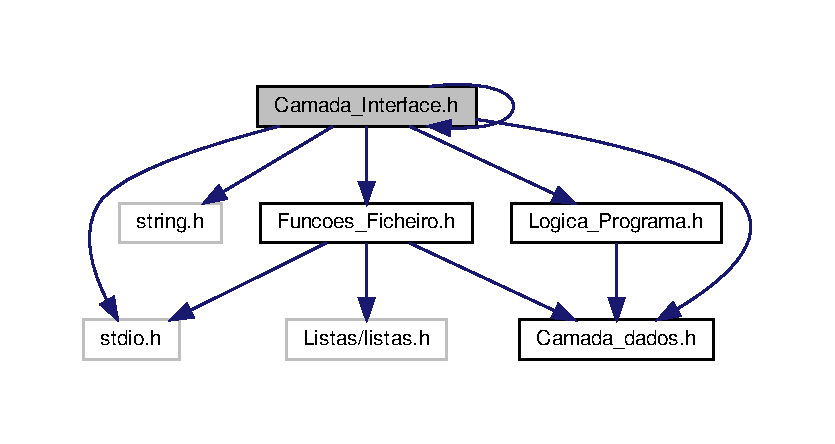
\includegraphics[width=350pt]{Camada__Interface_8h__incl}
\end{center}
\end{figure}
This graph shows which files directly or indirectly include this file\+:
\nopagebreak
\begin{figure}[H]
\begin{center}
\leavevmode
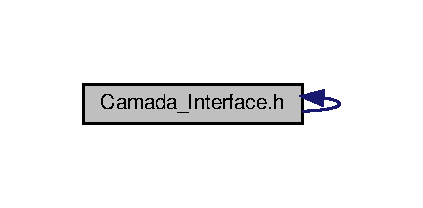
\includegraphics[width=203pt]{Camada__Interface_8h__dep__incl}
\end{center}
\end{figure}
\subsection*{Macros}
\begin{DoxyCompactItemize}
\item 
\mbox{\Hypertarget{Camada__Interface_8h_a6821bafc3c88dfb2e433a095df9940c6}\label{Camada__Interface_8h_a6821bafc3c88dfb2e433a095df9940c6}} 
\#define \hyperlink{Camada__Interface_8h_a6821bafc3c88dfb2e433a095df9940c6}{B\+U\+F\+\_\+\+S\+I\+ZE}~1024
\begin{DoxyCompactList}\small\item\em Definição do tamanho do buf. \end{DoxyCompactList}\end{DoxyCompactItemize}
\subsection*{Functions}
\begin{DoxyCompactItemize}
\item 
void \hyperlink{Camada__Interface_8h_a4525a57d0cd9ed3c9150e19b67e1dad6}{mostrar\+\_\+tabuleiro} (\hyperlink{structESTADO}{E\+S\+T\+A\+DO} $\ast$estado)
\begin{DoxyCompactList}\small\item\em Permite mostrar o tabuleiro. \end{DoxyCompactList}\item 
void \hyperlink{Camada__Interface_8h_a33d09196f922a638847c19f3aca3fc3c}{prompt} (\hyperlink{structESTADO}{E\+S\+T\+A\+DO} $\ast$e)
\begin{DoxyCompactList}\small\item\em Permite apresentar um prompt. \end{DoxyCompactList}\item 
int \hyperlink{Camada__Interface_8h_acdd45e696ba72db05e8e8937ba035cb5}{Resposta} (int resultado)
\begin{DoxyCompactList}\small\item\em Permite dar uma resposta no final do jogo. \end{DoxyCompactList}\item 
int \hyperlink{Camada__Interface_8h_a4c07684dcb63e1e1b3955a7d26481227}{jogar\+\_\+coord} (\hyperlink{structESTADO}{E\+S\+T\+A\+DO} $\ast$estado, \hyperlink{structCOORDENADA}{C\+O\+O\+R\+D\+E\+N\+A\+DA} coord)
\begin{DoxyCompactList}\small\item\em Joga uma coordenada. \end{DoxyCompactList}\item 
int \hyperlink{Camada__Interface_8h_a1d4126c044f8f4c350045d474a08019a}{movs} (\hyperlink{structESTADO}{E\+S\+T\+A\+DO} $\ast$estado)
\begin{DoxyCompactList}\small\item\em Mostra a lista de movimentos. \end{DoxyCompactList}\item 
int \hyperlink{Camada__Interface_8h_a24da95ebeede4a540e37790ce8be359b}{interpretador} (\hyperlink{structESTADO}{E\+S\+T\+A\+DO} $\ast$e)
\begin{DoxyCompactList}\small\item\em Interpretador. \end{DoxyCompactList}\end{DoxyCompactItemize}


\subsection{Detailed Description}
Definição do interpretador e mostrar tabuleiro e das funções associadas 

\subsection{Function Documentation}
\mbox{\Hypertarget{Camada__Interface_8h_a24da95ebeede4a540e37790ce8be359b}\label{Camada__Interface_8h_a24da95ebeede4a540e37790ce8be359b}} 
\index{Camada\+\_\+\+Interface.\+h@{Camada\+\_\+\+Interface.\+h}!interpretador@{interpretador}}
\index{interpretador@{interpretador}!Camada\+\_\+\+Interface.\+h@{Camada\+\_\+\+Interface.\+h}}
\subsubsection{\texorpdfstring{interpretador()}{interpretador()}}
{\footnotesize\ttfamily int interpretador (\begin{DoxyParamCaption}\item[{\hyperlink{structESTADO}{E\+S\+T\+A\+DO} $\ast$}]{e }\end{DoxyParamCaption})}



Interpretador. 


\begin{DoxyParams}{Parameters}
{\em e} & Apontador para o estado \\
\hline
\end{DoxyParams}
\begin{DoxyReturn}{Returns}
0 ou 1 
\end{DoxyReturn}
\mbox{\Hypertarget{Camada__Interface_8h_a4c07684dcb63e1e1b3955a7d26481227}\label{Camada__Interface_8h_a4c07684dcb63e1e1b3955a7d26481227}} 
\index{Camada\+\_\+\+Interface.\+h@{Camada\+\_\+\+Interface.\+h}!jogar\+\_\+coord@{jogar\+\_\+coord}}
\index{jogar\+\_\+coord@{jogar\+\_\+coord}!Camada\+\_\+\+Interface.\+h@{Camada\+\_\+\+Interface.\+h}}
\subsubsection{\texorpdfstring{jogar\+\_\+coord()}{jogar\_coord()}}
{\footnotesize\ttfamily int jogar\+\_\+coord (\begin{DoxyParamCaption}\item[{\hyperlink{structESTADO}{E\+S\+T\+A\+DO} $\ast$}]{estado,  }\item[{\hyperlink{structCOORDENADA}{C\+O\+O\+R\+D\+E\+N\+A\+DA}}]{coord }\end{DoxyParamCaption})}



Joga uma coordenada. 


\begin{DoxyParams}{Parameters}
{\em estado} & Apontador para o estado \\
\hline
{\em coord} & Apontador para a coordenada \\
\hline
\end{DoxyParams}
\begin{DoxyReturn}{Returns}
valor final (verdadeiro ou falso) 
\end{DoxyReturn}
\mbox{\Hypertarget{Camada__Interface_8h_a4525a57d0cd9ed3c9150e19b67e1dad6}\label{Camada__Interface_8h_a4525a57d0cd9ed3c9150e19b67e1dad6}} 
\index{Camada\+\_\+\+Interface.\+h@{Camada\+\_\+\+Interface.\+h}!mostrar\+\_\+tabuleiro@{mostrar\+\_\+tabuleiro}}
\index{mostrar\+\_\+tabuleiro@{mostrar\+\_\+tabuleiro}!Camada\+\_\+\+Interface.\+h@{Camada\+\_\+\+Interface.\+h}}
\subsubsection{\texorpdfstring{mostrar\+\_\+tabuleiro()}{mostrar\_tabuleiro()}}
{\footnotesize\ttfamily void mostrar\+\_\+tabuleiro (\begin{DoxyParamCaption}\item[{\hyperlink{structESTADO}{E\+S\+T\+A\+DO} $\ast$}]{estado }\end{DoxyParamCaption})}



Permite mostrar o tabuleiro. 


\begin{DoxyParams}{Parameters}
{\em estado} & Apontador para o estado \\
\hline
\end{DoxyParams}
\mbox{\Hypertarget{Camada__Interface_8h_a1d4126c044f8f4c350045d474a08019a}\label{Camada__Interface_8h_a1d4126c044f8f4c350045d474a08019a}} 
\index{Camada\+\_\+\+Interface.\+h@{Camada\+\_\+\+Interface.\+h}!movs@{movs}}
\index{movs@{movs}!Camada\+\_\+\+Interface.\+h@{Camada\+\_\+\+Interface.\+h}}
\subsubsection{\texorpdfstring{movs()}{movs()}}
{\footnotesize\ttfamily int movs (\begin{DoxyParamCaption}\item[{\hyperlink{structESTADO}{E\+S\+T\+A\+DO} $\ast$}]{estado }\end{DoxyParamCaption})}



Mostra a lista de movimentos. 


\begin{DoxyParams}{Parameters}
{\em estado} & Apontador para o estado \\
\hline
\end{DoxyParams}
\begin{DoxyReturn}{Returns}
0 
\end{DoxyReturn}
\mbox{\Hypertarget{Camada__Interface_8h_a33d09196f922a638847c19f3aca3fc3c}\label{Camada__Interface_8h_a33d09196f922a638847c19f3aca3fc3c}} 
\index{Camada\+\_\+\+Interface.\+h@{Camada\+\_\+\+Interface.\+h}!prompt@{prompt}}
\index{prompt@{prompt}!Camada\+\_\+\+Interface.\+h@{Camada\+\_\+\+Interface.\+h}}
\subsubsection{\texorpdfstring{prompt()}{prompt()}}
{\footnotesize\ttfamily void prompt (\begin{DoxyParamCaption}\item[{\hyperlink{structESTADO}{E\+S\+T\+A\+DO} $\ast$}]{e }\end{DoxyParamCaption})}



Permite apresentar um prompt. 


\begin{DoxyParams}{Parameters}
{\em e} & Apontador para o estado \\
\hline
\end{DoxyParams}
\mbox{\Hypertarget{Camada__Interface_8h_acdd45e696ba72db05e8e8937ba035cb5}\label{Camada__Interface_8h_acdd45e696ba72db05e8e8937ba035cb5}} 
\index{Camada\+\_\+\+Interface.\+h@{Camada\+\_\+\+Interface.\+h}!Resposta@{Resposta}}
\index{Resposta@{Resposta}!Camada\+\_\+\+Interface.\+h@{Camada\+\_\+\+Interface.\+h}}
\subsubsection{\texorpdfstring{Resposta()}{Resposta()}}
{\footnotesize\ttfamily int Resposta (\begin{DoxyParamCaption}\item[{int}]{resultado }\end{DoxyParamCaption})}



Permite dar uma resposta no final do jogo. 


\begin{DoxyParams}{Parameters}
{\em resultado} & Um inteiro \\
\hline
\end{DoxyParams}
\begin{DoxyReturn}{Returns}
Qual dos jogadores ganhou 
\end{DoxyReturn}

\hypertarget{Logica__Programa_8h}{}\section{Logica\+\_\+\+Programa.\+h File Reference}
\label{Logica__Programa_8h}\index{Logica\+\_\+\+Programa.\+h@{Logica\+\_\+\+Programa.\+h}}
{\ttfamily \#include \char`\"{}Camada\+\_\+dados.\+h\char`\"{}}\newline
Include dependency graph for Logica\+\_\+\+Programa.\+h\+:
\nopagebreak
\begin{figure}[H]
\begin{center}
\leavevmode
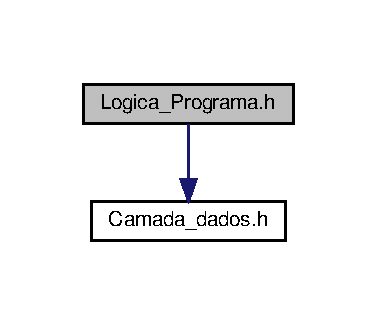
\includegraphics[width=181pt]{Logica__Programa_8h__incl}
\end{center}
\end{figure}
This graph shows which files directly or indirectly include this file\+:
\nopagebreak
\begin{figure}[H]
\begin{center}
\leavevmode
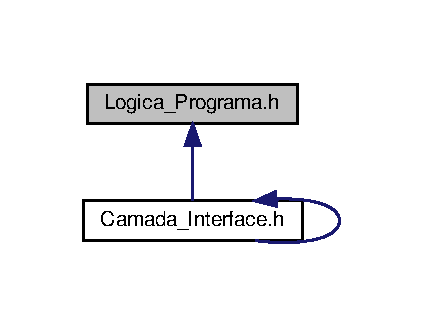
\includegraphics[width=203pt]{Logica__Programa_8h__dep__incl}
\end{center}
\end{figure}
\subsection*{Functions}
\begin{DoxyCompactItemize}
\item 
int \hyperlink{Logica__Programa_8h_a5c1d1c99ff9d180fb521119bdb4802cb}{e\+\_\+vizinha} (\hyperlink{structESTADO}{E\+S\+T\+A\+DO} $\ast$estado, \hyperlink{structCOORDENADA}{C\+O\+O\+R\+D\+E\+N\+A\+DA} coord)
\begin{DoxyCompactList}\small\item\em Testa se a Coordenada é vizinha da Coordenada anterior e se se encontra dentro do tabuleiro. \end{DoxyCompactList}\item 
int \hyperlink{Logica__Programa_8h_a58d9b18fb2ee96d48677648152f6dace}{possivel} (\hyperlink{structESTADO}{E\+S\+T\+A\+DO} $\ast$e, \hyperlink{structCOORDENADA}{C\+O\+O\+R\+D\+E\+N\+A\+DA} c)
\begin{DoxyCompactList}\small\item\em Testa se a jogada é possível. \end{DoxyCompactList}\item 
int \hyperlink{Logica__Programa_8h_a097ad6a7dc0606956897ad1c5d3a097a}{jogada\+\_\+valida} (\hyperlink{structESTADO}{E\+S\+T\+A\+DO} $\ast$estado, \hyperlink{structCOORDENADA}{C\+O\+O\+R\+D\+E\+N\+A\+DA} c)
\begin{DoxyCompactList}\small\item\em Testa se a Jogada é válida. \end{DoxyCompactList}\item 
int \hyperlink{Logica__Programa_8h_a065b9800844c5eac8568cfb601efc316}{cond\+\_\+canto} (\hyperlink{structCOORDENADA}{C\+O\+O\+R\+D\+E\+N\+A\+DA} c)
\begin{DoxyCompactList}\small\item\em Função que determina se a coordenada se encontra fora do tabuleiro. \end{DoxyCompactList}\item 
void \hyperlink{Logica__Programa_8h_a69eb26e048042f9beabd54d863d50599}{coordvizinho} (\hyperlink{structCOORDENADA}{C\+O\+O\+R\+D\+E\+N\+A\+DA} ls\mbox{[}$\,$\mbox{]}, \hyperlink{structCOORDENADA}{C\+O\+O\+R\+D\+E\+N\+A\+DA} c)
\begin{DoxyCompactList}\small\item\em Cria um array das coordenadas vizinhas. \end{DoxyCompactList}\item 
int \hyperlink{Logica__Programa_8h_a8656f33867e98b6c41bcc00f594c63e9}{vizivalide} (\hyperlink{structESTADO}{E\+S\+T\+A\+DO} $\ast$estado, \hyperlink{structCOORDENADA}{C\+O\+O\+R\+D\+E\+N\+A\+DA} coord)
\begin{DoxyCompactList}\small\item\em Testar se tem vizinhos validos. \end{DoxyCompactList}\item 
int \hyperlink{Logica__Programa_8h_a01b01396434b28ecd0f04546ebb28b1f}{fim} (\hyperlink{structESTADO}{E\+S\+T\+A\+DO} $\ast$estado, \hyperlink{structCOORDENADA}{C\+O\+O\+R\+D\+E\+N\+A\+DA} coord)
\begin{DoxyCompactList}\small\item\em Testa se a Coordenada é igual à final. \end{DoxyCompactList}\item 
int \hyperlink{Logica__Programa_8h_a53472e75f056ceb02b5387193021838a}{jogar} (\hyperlink{structESTADO}{E\+S\+T\+A\+DO} $\ast$estado, \hyperlink{structCOORDENADA}{C\+O\+O\+R\+D\+E\+N\+A\+DA} c)
\begin{DoxyCompactList}\small\item\em Modifica o estado ao jogar na casa correta se a jogada for válida. \end{DoxyCompactList}\end{DoxyCompactItemize}


\subsection{Detailed Description}
Definição da função jogar e funções associadas a essa 

\subsection{Function Documentation}
\mbox{\Hypertarget{Logica__Programa_8h_a065b9800844c5eac8568cfb601efc316}\label{Logica__Programa_8h_a065b9800844c5eac8568cfb601efc316}} 
\index{Logica\+\_\+\+Programa.\+h@{Logica\+\_\+\+Programa.\+h}!cond\+\_\+canto@{cond\+\_\+canto}}
\index{cond\+\_\+canto@{cond\+\_\+canto}!Logica\+\_\+\+Programa.\+h@{Logica\+\_\+\+Programa.\+h}}
\subsubsection{\texorpdfstring{cond\+\_\+canto()}{cond\_canto()}}
{\footnotesize\ttfamily int cond\+\_\+canto (\begin{DoxyParamCaption}\item[{\hyperlink{structCOORDENADA}{C\+O\+O\+R\+D\+E\+N\+A\+DA}}]{c }\end{DoxyParamCaption})}



Função que determina se a coordenada se encontra fora do tabuleiro. 


\begin{DoxyParams}{Parameters}
{\em c} & Apontador para coordenada \\
\hline
\end{DoxyParams}
\begin{DoxyReturn}{Returns}
1 ou 0 para verdadeiro ou falso 
\end{DoxyReturn}
\mbox{\Hypertarget{Logica__Programa_8h_a69eb26e048042f9beabd54d863d50599}\label{Logica__Programa_8h_a69eb26e048042f9beabd54d863d50599}} 
\index{Logica\+\_\+\+Programa.\+h@{Logica\+\_\+\+Programa.\+h}!coordvizinho@{coordvizinho}}
\index{coordvizinho@{coordvizinho}!Logica\+\_\+\+Programa.\+h@{Logica\+\_\+\+Programa.\+h}}
\subsubsection{\texorpdfstring{coordvizinho()}{coordvizinho()}}
{\footnotesize\ttfamily void coordvizinho (\begin{DoxyParamCaption}\item[{\hyperlink{structCOORDENADA}{C\+O\+O\+R\+D\+E\+N\+A\+DA}}]{ls\mbox{[}$\,$\mbox{]},  }\item[{\hyperlink{structCOORDENADA}{C\+O\+O\+R\+D\+E\+N\+A\+DA}}]{c }\end{DoxyParamCaption})}



Cria um array das coordenadas vizinhas. 


\begin{DoxyParams}{Parameters}
{\em ls} & array de coordenadas \\
\hline
{\em c} & Apontador para coordenada \\
\hline
\end{DoxyParams}
\mbox{\Hypertarget{Logica__Programa_8h_a5c1d1c99ff9d180fb521119bdb4802cb}\label{Logica__Programa_8h_a5c1d1c99ff9d180fb521119bdb4802cb}} 
\index{Logica\+\_\+\+Programa.\+h@{Logica\+\_\+\+Programa.\+h}!e\+\_\+vizinha@{e\+\_\+vizinha}}
\index{e\+\_\+vizinha@{e\+\_\+vizinha}!Logica\+\_\+\+Programa.\+h@{Logica\+\_\+\+Programa.\+h}}
\subsubsection{\texorpdfstring{e\+\_\+vizinha()}{e\_vizinha()}}
{\footnotesize\ttfamily int e\+\_\+vizinha (\begin{DoxyParamCaption}\item[{\hyperlink{structESTADO}{E\+S\+T\+A\+DO} $\ast$}]{estado,  }\item[{\hyperlink{structCOORDENADA}{C\+O\+O\+R\+D\+E\+N\+A\+DA}}]{coord }\end{DoxyParamCaption})}



Testa se a Coordenada é vizinha da Coordenada anterior e se se encontra dentro do tabuleiro. 


\begin{DoxyParams}{Parameters}
{\em estado} & Apontador para o estado \\
\hline
{\em coord} & A coordenada \\
\hline
\end{DoxyParams}
\begin{DoxyReturn}{Returns}
0 ou 1 para verdadeiro ou falso 
\end{DoxyReturn}
\mbox{\Hypertarget{Logica__Programa_8h_a01b01396434b28ecd0f04546ebb28b1f}\label{Logica__Programa_8h_a01b01396434b28ecd0f04546ebb28b1f}} 
\index{Logica\+\_\+\+Programa.\+h@{Logica\+\_\+\+Programa.\+h}!fim@{fim}}
\index{fim@{fim}!Logica\+\_\+\+Programa.\+h@{Logica\+\_\+\+Programa.\+h}}
\subsubsection{\texorpdfstring{fim()}{fim()}}
{\footnotesize\ttfamily int fim (\begin{DoxyParamCaption}\item[{\hyperlink{structESTADO}{E\+S\+T\+A\+DO} $\ast$}]{estado,  }\item[{\hyperlink{structCOORDENADA}{C\+O\+O\+R\+D\+E\+N\+A\+DA}}]{coord }\end{DoxyParamCaption})}



Testa se a Coordenada é igual à final. 


\begin{DoxyParams}{Parameters}
{\em estado} & Apontador para estado \\
\hline
{\em coord} & A coordenada \\
\hline
\end{DoxyParams}
\begin{DoxyReturn}{Returns}
0 ou 1 para verdadeiro ou falso 
\end{DoxyReturn}
\mbox{\Hypertarget{Logica__Programa_8h_a097ad6a7dc0606956897ad1c5d3a097a}\label{Logica__Programa_8h_a097ad6a7dc0606956897ad1c5d3a097a}} 
\index{Logica\+\_\+\+Programa.\+h@{Logica\+\_\+\+Programa.\+h}!jogada\+\_\+valida@{jogada\+\_\+valida}}
\index{jogada\+\_\+valida@{jogada\+\_\+valida}!Logica\+\_\+\+Programa.\+h@{Logica\+\_\+\+Programa.\+h}}
\subsubsection{\texorpdfstring{jogada\+\_\+valida()}{jogada\_valida()}}
{\footnotesize\ttfamily int jogada\+\_\+valida (\begin{DoxyParamCaption}\item[{\hyperlink{structESTADO}{E\+S\+T\+A\+DO} $\ast$}]{estado,  }\item[{\hyperlink{structCOORDENADA}{C\+O\+O\+R\+D\+E\+N\+A\+DA}}]{c }\end{DoxyParamCaption})}



Testa se a Jogada é válida. 


\begin{DoxyParams}{Parameters}
{\em estado} & Apontador para o estado \\
\hline
{\em c} & A coordenada \\
\hline
\end{DoxyParams}
\begin{DoxyReturn}{Returns}
0 ou 1 para verdadeiro ou falso 
\end{DoxyReturn}
\mbox{\Hypertarget{Logica__Programa_8h_a53472e75f056ceb02b5387193021838a}\label{Logica__Programa_8h_a53472e75f056ceb02b5387193021838a}} 
\index{Logica\+\_\+\+Programa.\+h@{Logica\+\_\+\+Programa.\+h}!jogar@{jogar}}
\index{jogar@{jogar}!Logica\+\_\+\+Programa.\+h@{Logica\+\_\+\+Programa.\+h}}
\subsubsection{\texorpdfstring{jogar()}{jogar()}}
{\footnotesize\ttfamily int jogar (\begin{DoxyParamCaption}\item[{\hyperlink{structESTADO}{E\+S\+T\+A\+DO} $\ast$}]{estado,  }\item[{\hyperlink{structCOORDENADA}{C\+O\+O\+R\+D\+E\+N\+A\+DA}}]{c }\end{DoxyParamCaption})}



Modifica o estado ao jogar na casa correta se a jogada for válida. 


\begin{DoxyParams}{Parameters}
{\em estado} & Apontador para o estado \\
\hline
{\em c} & A coordenada \\
\hline
\end{DoxyParams}
\begin{DoxyReturn}{Returns}
0 ou 1 para verdadeiro ou falso 
\end{DoxyReturn}
\mbox{\Hypertarget{Logica__Programa_8h_a58d9b18fb2ee96d48677648152f6dace}\label{Logica__Programa_8h_a58d9b18fb2ee96d48677648152f6dace}} 
\index{Logica\+\_\+\+Programa.\+h@{Logica\+\_\+\+Programa.\+h}!possivel@{possivel}}
\index{possivel@{possivel}!Logica\+\_\+\+Programa.\+h@{Logica\+\_\+\+Programa.\+h}}
\subsubsection{\texorpdfstring{possivel()}{possivel()}}
{\footnotesize\ttfamily int possivel (\begin{DoxyParamCaption}\item[{\hyperlink{structESTADO}{E\+S\+T\+A\+DO} $\ast$}]{e,  }\item[{\hyperlink{structCOORDENADA}{C\+O\+O\+R\+D\+E\+N\+A\+DA}}]{c }\end{DoxyParamCaption})}



Testa se a jogada é possível. 


\begin{DoxyParams}{Parameters}
{\em e} & Apontador para o estado \\
\hline
{\em c} & A coordenada \\
\hline
\end{DoxyParams}
\begin{DoxyReturn}{Returns}
0 ou 1 para verdadeiro ou falso 
\end{DoxyReturn}
\mbox{\Hypertarget{Logica__Programa_8h_a8656f33867e98b6c41bcc00f594c63e9}\label{Logica__Programa_8h_a8656f33867e98b6c41bcc00f594c63e9}} 
\index{Logica\+\_\+\+Programa.\+h@{Logica\+\_\+\+Programa.\+h}!vizivalide@{vizivalide}}
\index{vizivalide@{vizivalide}!Logica\+\_\+\+Programa.\+h@{Logica\+\_\+\+Programa.\+h}}
\subsubsection{\texorpdfstring{vizivalide()}{vizivalide()}}
{\footnotesize\ttfamily int vizivalide (\begin{DoxyParamCaption}\item[{\hyperlink{structESTADO}{E\+S\+T\+A\+DO} $\ast$}]{estado,  }\item[{\hyperlink{structCOORDENADA}{C\+O\+O\+R\+D\+E\+N\+A\+DA}}]{coord }\end{DoxyParamCaption})}



Testar se tem vizinhos validos. 


\begin{DoxyParams}{Parameters}
{\em estado} & Apontador para o estado \\
\hline
{\em coord} & Apontador para coordenada \\
\hline
\end{DoxyParams}
\begin{DoxyReturn}{Returns}
1 ou 0 para verdadeiro ou falso, respetivamente 
\end{DoxyReturn}

%--- End generated contents ---

% Index
\backmatter
\newpage
\phantomsection
\clearemptydoublepage
\addcontentsline{toc}{chapter}{Index}
\printindex

\end{document}
